\documentclass[11pt]{article}
\usepackage[includeheadfoot, top=1.0in, bottom=1.0in, hmargin=1.0in]{geometry}
\usepackage[utf8]{inputenc}
\usepackage{fancyhdr}
\usepackage{url}
\pagestyle{fancy}
\usepackage{setspace}
\usepackage{tabularx}
\usepackage{graphicx}
\usepackage{caption}
\usepackage{subcaption}
\usepackage{hyperref}
\usepackage{multicol}
\usepackage{amsmath}
\usepackage{enumitem}

\usepackage{hyperref}
\hypersetup{
    colorlinks=true,
    linkcolor=blue,
    filecolor=magenta,      
    urlcolor=blue,
}


\lhead{Astronomy Lab II}
\rhead{Spring 2022}
\lfoot{Mead / Yahalomi}
\rfoot{Mon 6-9pm}
\cfoot{\thepage}

\begin{document}

\begin{center}
\huge{Lab 8: Rules of Thumb \& Exploring the Night Sky}\\ \medskip \Large{March 28, 2022}
\end{center}

\section{Introduction}

In this lab, we will begin to learn how to navigate around the Night Sky.  First, we will come up with a ``handy'' way of measuring the size of distant objects.  Then we will test that method out.  We will also learn how to use a \textit{planisphere} to find constellations and then test how many of those we see outside.  Additionally, we will find out first hand just how many stars we DON'T see because of the lights of NYC.

\section{Handy Measurements}

Sextants allow the precise measurement of angles, but not all of us carry one in our back pocket (plus they take some practice). So you are going to calibrate various parts of your hand to allow you to measure angles.

\medskip \noindent
Extend your arm straight out from the shoulder. Now extend your thumb like you're hitchhiking. This will be one of your basic measuring devices. Now make a loose fist. There's your other device.

\medskip \noindent
\textbf{Record all your measurements and your calculations}

\begin{enumerate}
    \item Measure the width of your thumb across the nail using a ruler. With a partner, use a string or a yard stick to measure the distance from your eye to your thumb at arm's length. Get as accurate a measurement as possible. Check how much difference it makes if you hold your arm in front of you versus to the side, or move your head slightly. If r is the width of your thumb and D is the distance between your eye and thumb, calculate the angle subtended by your thumb in degrees using equation \ref{eq:small_angle}, and estimate (make a guess of) the precision in degrees of your measurement. Explain why you chose this value as your estimate.
    \begin{equation} \label{eq:small_angle}
        \theta \, \rm{(in \, degrees)} = \frac{r}{D} \times \frac{180^\circ}{\pi}
    \end{equation}
    \item Repeat this process for your fist (across the knuckles.)
    \item You now have two ``devices'' for estimating angles that are always with you. Use both of them to measure the angular size of a few things in the room.  Pick 2 not-too-big objects, stand a little distance away, and measure their angular size with both your fist and your thumb by counting how many fists and how many thumbs across the object is from where you are standing.
    \begin{enumerate}
        \item Then measure the distance from you to the object, and its actual size.
        \item Calculate the angular size as you did using equation \ref{eq:small_angle}, and check how close your hand estimates were to reality.
        \item Using equation \ref{eq:error}, calculate the percent error of the estimate you determined with your fist and with your thumb. Why might your estimate be inaccurate? Was your precision estimate from questions 1 and 2 close to correct?
    \end{enumerate}
    \begin{equation} \label{eq:error}
        \rm{percent \, error} = \frac{\rm{estimated \, value - true \, value}}{true \, value}
    \end{equation}
\end{enumerate}


\section{Making a Planisphere}

The \textbf{planisphere} is one of the handiest tools for a star-gazer. It was refined in Greece during the 4th century by Hypatia, a notable mathematician and astronomer of her day.  If you do not have one already, grab a planisphere handout.

\subsection{Construction}
\begin{enumerate}
    \item Identify which is the circular sky map and which is the star wheel's outer sleeve.
    \item Cut out the outermost circle on sky map.
    \item Cut out the outside border of the star wheel's outer sleeve.
    \item Cut out the shaded area at the center of the star wheel's outer sleeve.
    \item Fold the star wheel sleeve at the line over the star wheel.
    \item You will see a small clear circle at the center of sky map as well as at a point on the triangle that you've folded over. Attach the plates with a pin through the centers (marked by these clear circles) so they are centered and can rotate freely. Bend the pin so the point lies flat against the back of the bottom plate, and tape it there.
\end{enumerate}

A planisphere works as follows: align the planisphere window such that the time you are interested in (generally the current time) matches with the date you are interested in (generally the current date). Then, by looking in the window of the planisphere, we can see the constellations that we expect in the night sky at a given time on a given date. On a planisphere, the brightness of a star is represented by the size of its dot. Usually a few dots sizes are used on the star map, each corresponding to a different range of brightness, or \textit{magnitude}.

\subsection{Using the Planisphere}
\begin{enumerate}
    \item What happens to the number of stars you see of a given brightness as you consider dimmer and dimmer magnitudes?
    \item Why does the star count depend on brightness like this? To simplify this problem, assume for a minute that all stars give off the same amount of light.  Draw a diagram if you think it will aid your explanation.
    \item Five of the planets in the sky are bright enough to outshine a lot of stars shown on the planisphere. \textbf{Why aren't the planets mapped?} Hint: the word ``planet'' is derived from the Greek word for ``wanderer''.
    \item Look up Regulus online, what constellation is it in? Label it on your planisphere. Using your planisphere, answer the following questions: When does Regulus set today? When does it set a month from now?
    \item Look up Spica online, what constellation is it in? Label it on your planisphere. Using your planisphere, answer the following questions: When does Spica set today? When does it set a month from now?
    \item Look up Polaris online, what constellation is it in? Label it on your planisphere. Using your planisphere, answer the following questions: When does Polaris set today? When does it set a month from now? Hint: Polaris is also known as the North Star.
    \item Based on Figure \ref{fig: altitude}, what would Polaris' altitude be if you were standing at the North Pole?
    \item Based on Figure \ref{fig: altitude}, what would Polaris' altitude be if you were standing at the equator?
    \item Why does the pin go through the North Star?  What aspect of the Earth's geometry/rotation is responsible for this?
\end{enumerate}


\begin{figure}[htb!] 
\center
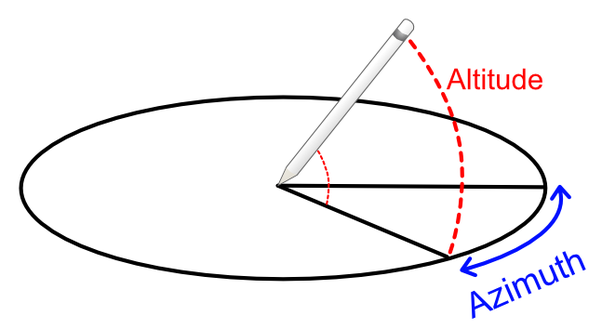
\includegraphics[width=15cm]{Images/altitude.png}
\caption{Altitude and Azimuth in astronomy.}
\label{fig: altitude}
\end{figure}

\subsection{Part III --- Outdoor Observing}

Using your fist, we'll try to measure how a star moves. 

\begin{enumerate}
    \item With your planisphere, orient yourself and identify as many constellations as you can from the roof.  Write them down in your notebook.  \textbf{In what part of the sky is it easiest for you to see stars, and why? What effect does the Moon have on the visibility of stars and constellations?}
    \item Find Polaris, the North Star. \textbf{Face it and measure its altitude using your thumb or fist?} How does Polaris' altitude relate to NYC's latitude (40$^{\circ}$)? Why does this make sense (hint: Polaris' latitude is 90$^{\circ}$ and think back to the previous questions about Polaris' altitude that you answered)?
    \item Pick a star near the Eastern or Western horizon.  Make sure it's bright enough that you can find it easily an hour from now. Also, make sure it is not a planet (we can help you with this). Make a note on your planisphere if necessary. \textbf{Measure the altitude, first with your fist, then with your thumb.  Which do you think is more accurate? Why? Note the time.}
    \item How do you expect the altitude of your star to change over the next hour? Draw a diagram to explain.
\end{enumerate}

\medskip \noindent
We will now spend a little time looking at the Moon (and maybe a star cluster if it is visible through clouds and moonlight).  \textbf{Draw one largish circle per object we observe in your notebook.}  Each one will be used to draw the field of view for a particular object. When looking through the telescope, and right afterwards, make a neat drawing of what you see. \textbf{Draw what you actually see, perhaps making brighter stars a little larger or indicate their brightness with some other label. Label everything. Can you identify the constellations that these objects are in or near?}

\medskip \noindent
Next we will estimate the number of stars that we can't see by being in New York City and because of the Moon.  Find a star in the night sky. Based on the planisphere, try to identify what star it is. \textbf{Note what star you picked. Can you see the star clearly? Can you see the other stars in it's constellation clearly? How many stars can you see in this field of view?}

\medskip \noindent
In this field of view, one can potentially see 14,000 stars. In general, the fainter the stars that you can see, the more you can see.  They follow the following trend:

\begin{center}
\begin{tabular}{|c|c|}
\hline
Limiting & Number\\
Magnitude & Of Stars\\
\hline
1 & 6\\
2 & 45\\
3 & 150\\
4 & 540\\
5 & 1700 \\
6 & 4900\\
7 & 14000\\
\hline
\end{tabular}
\end{center}

\noindent
Based on the magnitude chart above, \textbf{how many stars were you NOT able to see tonight because of the lights of the city?  Where did you grow up?  Can you guess about what limiting magnitude the sky by your hometown is?  How many more stars can you see there than in New York City?}

\medskip \noindent
\textbf{Finally, back to the altitude of your star:}

\begin{enumerate}[resume]
    \item Later on: note the time again. What is the altitude of the star now, measured just using your fist or thumb?
    \item What was the angular rate of rotation of the star near the horizon in degrees per hour? (hint: we measured the altitude at two times, so by taking the difference of the altitudes divided by the difference in the times, we can determine the angular rate of rotation!)
    \item In one day, a star should rotate 360$^{\circ}$. Do you find that if you convert your angular rate of rotation to degrees per day?
\end{enumerate}


\end{document}

